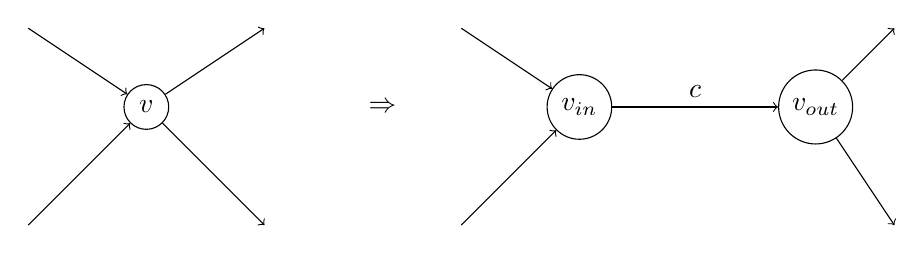
\begin{tikzpicture}
\tikzstyle{ver} = [circle, draw];

\node[ver] (v1) at (0.5,0) {$v$};
\draw (-1,1) edge[->] (v1);
\draw (-1,-1.5) edge [->](v1);
\draw (v1) edge [->](2,1);
\draw (v1) edge [->](2,-1.5);

\node at (3.5,0) {$\Rightarrow$};

\node [ver] (v2) at (6,0) {$v_{in}$};
\node [ver] (v3) at (9,0) {$v_{out}$};
\draw[->]  (v2) edge node[above] {$c$} (v3);
\draw (4.5,1) edge [->](v2);
\draw (4.5,-1.5) edge [->](v2);
\draw (v3) edge [->](10,1);
\draw (v3) edge [->](10,-1.5);
\end{tikzpicture}
